\label{sec:functionality}
%
It is noteworthy to introduce some concepts, techniques and tools that constitute the conceptual and functional background of this work.
%
These are essential to understand how the contributions work.

%Before going further in the presentation of \RenewGrass{} it is necessary to introduce some concepts, techniques and tools that constitute the conceptual and functional background of this work.
%
\subsection{Cloud Computing}
%
Cloud computing is a model for enabling ubiquitous, convenient, on-demand network access to a shared pool of configurable computing resources (e.g., networks, servers, storage, applications, and services).
%
Cloud computing can be viewed as a collection of services, which can be presented as a set of loosely-coupled layers \cite{Mell+11}.
%
These service models are closely related and can be seen as three layers, which are the Infrastructure as a Service (IaaS), the Software as a Service (SaaS) and the Platform as a Service (PaaS).
%
Before the emergence of the Cloud technology, there were significant research projects dealing with the development of distributed and scientific workflow systems with the grid paradigm. 
%
Workflow enactment service can be built on top of the low level grid middle-ware (eg. Globus Toolkit\footnote{http://www.globus.org/toolkit/}, UNICORE\footnote{http://www.unicore.eu/}, EGI \footnote{https://www.egi.eu/} and Alchemi\footnote{http://www.cloudbus.org/$ \sim $alchemi/}), through which the workflow management system invokes services provided by grid resources \cite{YuB05}.
%
At both the build-time and run-time phases, the state of the resources and applications can be retrieved from grid information services. 
%
There are many grid workflow management systems in use; like these representative projects: ASKALON \footnote{\url{http://www.askalon.org/}}, Pegasus \footnote{\url{http://www.pegasus.org/}}, Taverna \footnote{\url{http://www.taverna.org.uk/}}, Kepler\footnote{\url{https://kepler-project.org/}}, Triana\footnote{\url{http://www.trianacode.org/}} and Swift \cite{Zhao+11}.
%
Most of these projects, have been investigating the adaptation of their architectures to include the Cloud technology.
%
For instance, the Elastic Compute Cloud (EC2) module has been implemented to make Kepler supports Amazon Cloud services.
%
Launched in 2012, the Amazon Simple Workflow (SWF)\footnote{aws.amazon.com/swf} is an orchestration service for building scalable applications.
%
It maintains the execution state of the workflow in terms of consistency and reliability.
%
It permits structuring the various processing steps in an application running on one or more systems as a set of tasks.
%
These systems can be Cloud-based, on-premise, or both. But they lack of use of standard specification tools and notations. Contrarily to Petri-nets, The specification tolls  of these present also the disadvantage of missing a verifying tool.
\subsection{Reference Nets}
%
As stated above, we use Petri nets and more specifically \textit{reference nets} \cite{Kummer02}.%, which are well-founded modeling and analyzing technique of distributed systems. 
%
The latter extend the colored Petri net formalism by combining the concepts of synchronous channels.
%
Reference nets are the implementation of the concept of \emph{nets-within-nets} \cite{Valk98}, which allows tokens to be nets again.
%
With \textit{reference nets}, Petri nets are not only useful for modeling and analyzing of systems but also for implementation.
%
Their advantage is that the model is transformed into an implementation without changing the formalism.
%
Thus, the gap between modeling and implementation is diminished \cite{Cabac09c}.
%
%The main advantage of reference nets lies in the use of Java inscriptions within the transitions making the gap between specification and implementation decrease considerably.
%
Reference nets are object-oriented high-level Petri nets and are based on the nets-within-nets formalism introduced by \cite{Valk98}, which allows tokens to be nets again.
%
They extend Petri nets with dynamic net instances, net references, and dynamic transition synchronization through synchronous channels. Reference nets consist of places, transitions and arcs. 
%
The input and output arcs have a similar behavior to ordinary Petri nets. 
%
Tokens can be available of any type  in the Java programming language.
%
In opposite to the net elements of P/T nets, reference nets provide supplementary elements that increase the modeling power. 
%
These elements are: virtual places, declaration and arc types.
%
The places are typed and the transitions can hold expressions, actions, guards, etc.
%
Firing a transition can also create a new instance of a subnet.
%
The creation of the instances is similar to object instances in object-oriented programming.
%
This allows a specific, hierarchical nesting of networks, which is helpful for building complex systems.

The nets shown in Fig.~\ref{figure:refnets} are to illustrate two important features of reference nets, which are the notion of \emph{synchrnous channels} and net inscription (Java).
%
These two features are used frequently in this work.
%
The figure shows the modeling of a simple Cloud-based storage workflow.
%
The model is composed of two different nets that need to communicate with each other in order to store files in the Cloud using a Cloud service (DropBox).
%
The net (a) represents the Web authentication step to the DropBox service\footnote{https://www.dropbox.com/}.
%
It consists on setting the user credentials up.
%
This is performed by creating an instance of the Java class \textit{DropTransition} and checking the credentials by calling the method \emph{connect()}.
%
If the above step succeeds, then a URL\footnote{The generated url is the IP address of the authentication page of the DropBox service.} is generated. 
%
After completion, Net (a) creates a new instance of Net (b), which will use the generated information from Net (a) to upload files to the repository.
%
This is performed by using synchronous channels (down and up-links).

\begin{figure}[!t]
 \centering
  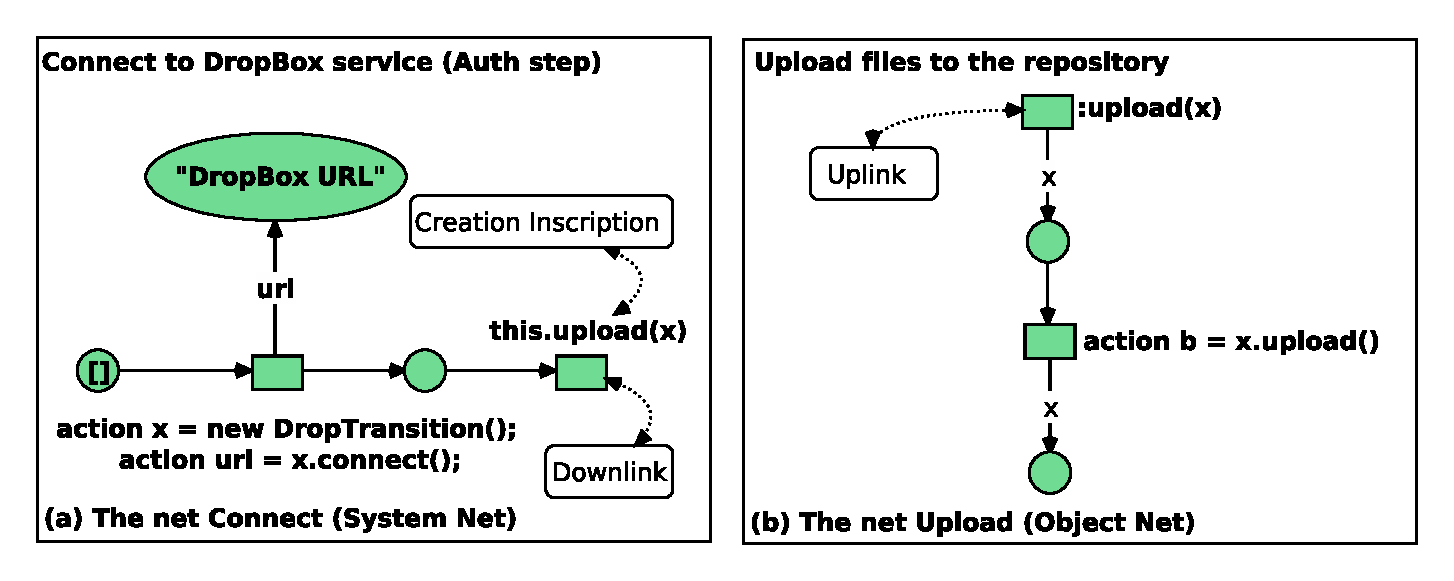
\includegraphics[width=0.79\textwidth,height=0.23\textheight]{images/SystemObjectNet}
\caption{(a) The System Net, (b) The Sub-net Upload}
\label{figure:refnets}
\end{figure}




%Renew 

\subsection{\Renew{}}
%
The \textbf{RE}ference \textbf{NE}ts \textbf{W}orkshop (\Renew{}), which is available at (\url{http://www.renew.de/}) is a graphical tool for creating, editing and simulating reference nets.
%
It combines the \textit{nets-within-nets} paradigm with the implementing power of Java.
%
%
%
With \Renew{} it is possible to draw and simulate both Petri nets and reference nets. 
%
%
%
During the simulation, a net instance is created and can be viewed in a separate window as its active transitions fire.
%
Simulation is used in Renew to view firing sequences of active transitions in reference nets.
%
Simulation can run in a one step modus where users can progress in steps where only one transition fires. 
%
\Renew{} also offers the possibility to set breakpoints to hold the simulation process.
%
Breakpoints can be set to places and transitions. 
%
By changing the compiler, \Renew{} can also simulate P/T nets, timed petri nets, Workflow nets, etc.

\Renew{} is an editor as well as a simulator for Petri nets and \textit{reference nets}.
%%Plug-in system
Since the version 1.7, \Renew{} is built on a highly sophisticated plug-in architecture, which was developed and introduced in \cite{Schleinzer+08}.
%
It allows the extension of \Renew{} with additional functionality through the use of interfaces from \Renew{} components without changing the core of \Renew{}.

%\subsection{Objectives}
%
\subsection{The Grass GIS}
%
\label{subsec:grassgis}
%Here we give an overview of the Grass GIS.
%
Grass is a multi-purpose open source GIS, which can be used for geoprocessing applications such as: geospatial data production, analysis and mapping. 
%
It can handle raster as well vector data.
%
The most important specificity of the Grass GIS is its modularity, which diminishes overhead.
%
This allows to run only the required modules (same as \Renew{}).
%
These modules are organized in categories (general GIS modules, raster modules, vector modules, etc.).
%
Table. \ref{tab:grasscommands} shows the modules provided by the Grass GIS \cite{Neteler+12}.

\begin{table}[!t]
\renewcommand{\arraystretch}{1.3}
\caption{Grass GIS Commands (from \cite{Neteler+12})}
\label{tab:grasscommands}
\centering
\begin{tabular}{c||c||c}
\hline
\bfseries Prefix & \bfseries Function class & \bfseries Type of command\\
\hline\hline
d.* & display & graphical output\\
\hline\hline
db.* & database & database management\\
\hline\hline
g.* & general & general file operations\\
\hline\hline
i.* & imagery & image processing\\
\hline\hline
m.* & misc & miscellaneous commands\\
\hline\hline
ps.* & postscript & map creation in Postscript format\\
\hline\hline
r.* & raster & 2D raster data processing\\
\hline\hline
r3.* & 3D raster & 3D raster data processing\\
\hline\hline
v.* & vector & 2D and 3D vector data processing\\
\hline
\end{tabular}
\end{table}


In order to allow \Renew{} executing these commands directly from the Petri net transitions, \RenewGrass{} offers a wrapping layer, which makes the Grass modules available at runtime.
%
Before using the modules for processing the data, the latter should be first imported into a Grass \textit{DATABASE}.\\
%
Within the DATABASE, the projects are organized as subdirectories called "LOCATIONS".
%
Each LOCATION can have one or more MAPSETS. 
%
Each \textit{MAPSET} may represent a sub region within a given LOCATION.
%
These are mostly the important variables that need to be set.




